\documentclass[12pt]{article}
\usepackage{epsf,epic,eepic,eepicemu}
%\documentstyle[epsf,epic,eepic,eepicemu]{article}
\usepackage[utf8]{inputenc}
\usepackage[czech]{babel}     
\usepackage{ae}
\usepackage{fancyhdr}

\usepackage[dvipdfm]{graphicx}
\author{Martin Venuš, Jaroslav Líbal}

\graphicspath{{img/}}

\usepackage[dvipdfm,unicode,colorlinks]{hyperref}
\hypersetup{bookmarksopen=false,hypertexnames=false, anchorcolor=black, citecolor=black, filecolor=black, linkcolor=black, menucolor=black, urlcolor=blue, pdfauthor={Martin Venuš, Jaroslav Líbal}, pdftitle={Závěrečná zpráva - semestrální projekt MI-PAR}}

\begin{document}
%\oddsidemargin=-5mm \evensidemargin=-5mm \marginparwidth=.08in
%\marginparsep=.01in \marginparpush=5pt \topmargin=-15mm
%\headheight=12pt \headsep=25pt \footheight=12pt \footskip=30pt
%\textheight=25cm \textwidth=17cm \columnsep=2mm \columnseprule=1pt
%\parindent=15pt\parskip=2pt

% ============================ Hlavička dokumentu ==================================================================
\begin{center}
\bf Semestrální projekt MI-PAR 2010/2011\\[5mm]
    Paralelní algoritmus pro řešení problému\\[5mm]
       Jaroslav Líbal\\
       Martin Venuš\\[5mm]
FIT ČVUT\\[2mm]
magisterské studijum\\[2mm]
Kolejní 550/2, 160 00 Praha 6\\[2mm]
29. listopadu 2010
\end{center}

%\pagestyle{empty} %get rid of header/footer for toc page
\newpage
\tableofcontents
\newpage
%\pagestyle{fancy}

% ============================ Definice problému a popis sekvenčního algoritmu ==================================================================
\section{Zadání úlohy}
\textbf{Úloha MBG: minimální obarvení grafu}

\subsection{Vstupní data}

$G(V,E)$ = jednoduchý neorietovaný neohodnocený k-regulární graf o~n uzlech a m hranách\\
$n$ = přirozené číslo představující počet uzlů grafu G, $n \geq 5$
$k$ = přirozené číslo řádu jednotek představující stupeň uzlu grafu G, $n \geq k \geq 3$; n a k~nejsou současně obě liché\\
\\
Doporučení pro generování G:\\
\\
Použijte generátor grafu s~volbou typu grafu "-t REG", který vygeneruje souvislý neorientovaný neohodnocený graf.


\subsection{Úkol} 

Nalezněte minimální uzlové obarvení grafu G, či-li zobrazení B: V~$\rightarrow$ N takové, že b=$\left|\{B[x]; x\ in\ V\}\right|$ je minimální. Řešení existuje vždy, nemusí být jednoznačné.

\subsection{Výstup algoritmu}

Počet použitých barev a výpis uzlového obarvení $B[1..n]$ grafu G ve formě matice sousednosti (barvy uzlů pište na diagonálu matice).\\

\subsection{Sekvenční algoritmus}

Sekvenční algoritmus je typu BB-DFS s~omezenou hloubkou prohledávaného prostoru. Cena, kterou minimalizuje, je počet barev b. Mezistav je dán částečným obarvenim. Mezistav či koncový stav je přípustný, jestliže žádné 2 sousední uzly nejsou obarvené stejnou barvou. Návrat v~mezistavu provádíme, pokud nelze žádný neobarvený uzel obarvit, aniž by se porušila podminka uzlového barvení.\\
\\
Triviální horní mez na $b=k+1$ (každý k-regulární graf lze uzlově obarvit $k+1$ barvami).\\
Těsná spodní mez na $b=2$. Pokud je G bipartitní, existuje obarvení dvěma barvami.


\subsection{Paralelní algoritmus}

Paralelní algoritmus je typu G-PBB-DFS-D. 

% ============================ Implementace ==================================================================
\section{Implementace}

\subsection{Sekvenční algoritmus}
Sekvenční algoritmus byl implementován přesně dle zadání. Vstupem programu je matice vygenerovaná programem \texttt{generator} s parametrem \texttt{-t REG}. Výstup algoritmu je následující:
\begin{itemize}
\item informace o minimálním počtu použitých barev (např. Pocet pouzitych barev: 8)
\item matice, která má na hlavní diagonále obarvení (číslo barvy) jednotlivých vrcholů
\item čas běhu algoritmu (např. Proces pracoval 376.300000 sekund.)
\end{itemize}

Příklad výstupu:
\begin{verbatim}
Pocet pouzitych barev: 2
001
001
111
Proces pracoval 0.000000 sekund.
\end{verbatim}

Časy běhu algoritmu pro různě velká data jsou uvedeny v tabulce č. \ref{doba_behu_sekvencne}.

% ============================ Paralelní algoritmus ==================================================================
\subsection{Paralelní algoritmus}

Před započetím vlastního paralelního výpočtu je procesorem s identifikátorem 0 načtena vstupní matice, která je spolu s informací o počtu jejich vrcholů distribuována pomocí příkazu \textbf{MPI\_Bcast} všem ostatním aktivním procesorům. Každý z procesorů následně provede inicializaci svého lokálního zásobníku a může být zahájen paralelní výpočet.

Výpočet paralelního algoritmu procesorem P0 začíná shodně se sekvenčním řešením - procesor vezme první vrchol vstupní matice, nalezne všechny jeho sousedy a ty vloží do zásobníku. V případě, že již nalezl všechny sousedy pak daný vrchol obarví. Poté co provedl obarvení prvního vrcholu začíná výpočet v hlavní smyčce programu. Ostatní procesory aktivně čekají a ptají se ostatních procesorů na práci.

\subsubsection{Hlavní smyčka algoritmu}

Hlavní smyčka programu je naznačena na obrázku v příloze (\ref{hlavniSmycka}). Každý procesor, který má práci, nejprve po obarvení vrcholu obslouží všechny požadavky na práci které obdržel. Pokud již vygeneroval více než jedno dílčí řešení, rozdělí tato řešení na dvě části. První polovinu si ponechá a druhou polovinu odešle spolu se zásobníkem všech doposud objevených vrcholů žádajícímu procesoru. V případě, že již nemá dostatek práce k odeslání odpoví, že nemá žádnou práci k předání a dále pak rozvíjí své poslední dílčí řešení stejným způsobem jako v sekvenčním algoritmu.

V okamžiku kdy procesoru dojde práce a tedy rozvinul všechna svá dílčí řešení, uloží si nejlepší z nich a postupně žádá všechny ostatní procesory o práci dokud ji neobdrží nebo nebyl paralelní výpočet ukončen.

\subsubsection{Ukončení paralelního výpočtu}

Iniciovat ukončení paralelního výpočtu může pouze procesor P0. V případě, že procesoru P0 došla práce a jeho požadavky na její přidělení byly opakovaně odmítány, nastaví svou barvu na bílou a pošle peška bílé barvy procesoru P1. Jestliže procesor Pi posílá práci procesoru Pj, kde i>j, pak Pi nastaví svou barvu na hnědou. Ve chvíli kdy procesoru Pi dojde práce, kontroluje příchod peška a v případě že jej obdrží, nastaví barvu peška podle své barvy (z hnědé barvy vytvoří černou) a odešle jej po kružnici procesoru Pi+1. Po odeslání peška se z hnědé barvy stává bílá. Pokud P0 obdrží zpět peška bílé barvy, je možné výpočet ukončit (o tomto informuje všechny ostatní procesory vysláním speciální zprávy), jinak ještě některý z procesorů pracuje a je nutné možnost ukončení algoritmu ověřit znovu později.

\subsubsection{Používané konstanty (tagy) ve zprávách}
\begin{description}
\item[MESSAGE\_MATRIX] odesílání vstupní matice
\item[MESSAGE\_JOB\_REQUIRE] žádost o práci
\item[MESSAGE\_JOB\_REQUIRE\_ANSWER] odpověď na žádost o práci
\item[MESSAGE\_JOB\_REQUIRE\_COLORS] odesíláme počet barev konfigurace
\item[MESSAGE\_JOB\_REQUIRE\_CONFIGURATION\_ARRAY] odesíláme konfiguraci
\item[MESSAGE\_JOB\_REQUIRE\_ITEMS] odesíláme počet prvků v konfiguraci
\item[MESSAGE\_JOB\_REQUIRE\_STACK\_SIZE] odesíláme velikost zásobníku
\item[MESSAGE\_JOB\_REQUIRE\_STACK\_TOP] odesíláme vrchol zásobníku
\item[MESSAGE\_JOB\_REQUIRE\_STACK\_ARRAY] odesíláme zásobník
\item[MESSAGE\_JOB\_REQUIRE\_DIAG] odesíláme diagonálu matice
\item[MESSAGE\_JOB\_REQUIRE\_CONFIGURATION\_ARRAY\_SIZE] odesíláme velikost pole konfigurací
\item[PESEK] odesíláme testovacího peška
\item[PESEK\_FINAL] odesíláme ukončovacího peška
\item[MESSAGE\_FINISH\_BEST\_COLORS] procesor odesílá své nejlepší chromatické číslo
\item[MESSAGE\_FINISH\_BEST] odesíláme číslo procesoru s nejlepší konfigurací
\end{description}

\subsubsection{Konstanty pro barvy peška a procesoru}
\begin{description}
\item[PESEK\_WHITE] bílá
\item[PESEK\_BLACK] černá
\item[PESEK\_BROWN] hnědá
\end{description}

% ============================ Naměřené výsledky a vyhodnocení ==================================================================
\section{Naměřené výsledky a vyhodnocení}

\subsection{Zadání měření}
\begin{enumerate}
\item Zvolte tři instance problému s~takovou velikostí vstupních dat, pro které má
sekvenční algoritmus časovou složitost kolem 5, 10 a 15 minut. Pro
meření čas potřebný na čtení dat z~disku a uložení na disk
neuvažujte a zakomentujte ladící tisky, logy, zprávy a výstupy.
\item Měřte paralelní čas při použití $i=2,\cdot,32$ procesorů na sítích Ethernet a InfiniBand.
%\item Pri mereni kazde instance problemu na dany pocet procesoru spoctete pro vas algoritmus dynamicke delby prace celkovy pocet odeslanych zadosti o praci, prumer na 1 procesor a jejich uspesnost.
%\item Mereni pro dany pocet procesoru a instanci problemu provedte 3x a pouzijte prumerne hodnoty.
\item Z~naměřených dat sestavte grafy zrychlení $S(n,p)$. Zjistěte, zda a za jakych podmínek
došlo k~superlineárnímu zrychlení a pokuste se je zdůvodnit.
\item Vyhodnoďte komunikační složitost dynamického vyvažování zátěže a posuďte
vhodnost vámi implementovaného algoritmu pro hledání dárce a dělení
zásobníku pri řešení vašeho problému. Posuďte efektivnost a
škálovatelnost algoritmu. Popište nedostatky vaší implementace a
navrhněte zlepšení.
\item Empiricky stanovte
granularitu vaší implementace, tj., stupeň paralelismu pro danou
velikost řešeného problému. Stanovte kritéria pro stanovení mezí, za
kterými již není učinné rozkládat výpočet na menší procesy, protože
by komunikační náklady prevážily urychlení paralelním výpočtem.
\end{enumerate}

\subsection{Matice pro měření}
Pro měření výsledků byly vygenerovány následující matice:
\begin{table}[ht]
\centering
\begin{tabular}{|l|c|c|c|c|}
\hline \textbf{Matice} & \textbf{Typ matice} & \textbf{Počet vrcholů} & \textbf{Stupeň vrcholu} \\
\hline 
\hline Matice 1 & REG & 42 & 18 \\ 
\hline Matice 2 & REG & 44 & 29 \\ 
\hline Matice 3 & REG & 43 & 12 \\ 
\hline 
\end{tabular}
\caption{Popis jednotlivých vygenerovaných matic.}
\label{matice_popis}	
\end{table}

REG = k-regulární graf

\subsection{Sekvenční řešení}

\begin{table}[ht]
\centering
\begin{tabular}{|l|c|c|c|c|}
\hline \textbf{Typ matice} & \textbf{čas 1 [s]} & \textbf{čas 2 [s]} & \textbf{čas 3 [s]} & \textbf{prům. čas [s]} \\
\hline 
\hline Matice 1 & 364.7 & 364.9 & 365.0 & \textbf{364.86} \\ 
\hline Matice 2 & 652.3 & 651.5 & 651.4 & \textbf{651.70} \\ 
\hline Matice 3 & 1184.7 & 1184.0 & 1184.9 & \textbf{1184.53} \\ 
\hline 
\end{tabular}
\caption{Doba běhu sekvenčního algoritmu pro jednotlivé matice.}
\label{doba_behu_sekvencne}	
\end{table}

%\newpage
\subsection{Paralelní řešení}
\begin{table}[ht]
\centering
\begin{tabular}{|l|c|c|c|c|}
\hline \textbf{Typ matice} & \textbf{Počet procesorů} & \textbf{čas - ethernet [s]} & \textbf{čas - infiniband [s]} \\
\hline 
\hline Matice 1 & 2 & 0.293 & 0.237 \\ 
\hline Matice 2 & 2 & 0.486 & 0.473 \\ 
\hline Matice 3 & 2 & 0.361 & 0.361 \\ 
\hline
\hline Matice 1 & 4 & 0.240 & 0.325 \\ 
\hline Matice 2 & 4 & 0.553 & 0.550 \\ 
\hline Matice 3 & 4 & 0.419 & 0.362 \\ 
\hline 
\hline Matice 1 & 8 & 0.290 & 0.254 \\ 
\hline Matice 2 & 8 & 0.382 & 0.573 \\ 
\hline Matice 3 & 8 & 0.359 & 0.595 \\ 
\hline 
\hline Matice 1 & 12 & 0.355 & 0.178 \\ 
\hline Matice 2 & 12 & 0.206 & 0.332 \\ 
\hline Matice 3 & 12 & 0.264 & 0.229 \\ 
\hline 
\hline Matice 1 & 16 & 0.237 & 0.374 \\ 
\hline Matice 2 & 16 & 0.590 & 0.398 \\ 
\hline Matice 3 & 16 & 0.326 & 0.515 \\ 
\hline 
\hline Matice 1 & 24 & 1.146 & 0.757 \\ 
\hline Matice 2 & 24 & 0.368 & 0.853 \\ 
\hline Matice 3 & 24 & 0.752 & 0.862 \\ 
\hline 
\end{tabular}
\caption{Doba běhu paralelního algoritmu.}
\label{doba_behu_paralelne}	
\end{table}


\subsubsection{Grafy zrychlení paralelního řešení}
% GNUPLOT: LaTeX picture
\setlength{\unitlength}{0.240900pt}
\ifx\plotpoint\undefined\newsavebox{\plotpoint}\fi
\sbox{\plotpoint}{\rule[-0.200pt]{0.400pt}{0.400pt}}%
\begin{picture}(1500,900)(0,0)
\sbox{\plotpoint}{\rule[-0.200pt]{0.400pt}{0.400pt}}%
\put(211.0,131.0){\rule[-0.200pt]{4.818pt}{0.400pt}}
\put(191,131){\makebox(0,0)[r]{ 200}}
\put(1429.0,131.0){\rule[-0.200pt]{4.818pt}{0.400pt}}
\put(211.0,196.0){\rule[-0.200pt]{4.818pt}{0.400pt}}
\put(191,196){\makebox(0,0)[r]{ 400}}
\put(1429.0,196.0){\rule[-0.200pt]{4.818pt}{0.400pt}}
\put(211.0,260.0){\rule[-0.200pt]{4.818pt}{0.400pt}}
\put(191,260){\makebox(0,0)[r]{ 600}}
\put(1429.0,260.0){\rule[-0.200pt]{4.818pt}{0.400pt}}
\put(211.0,325.0){\rule[-0.200pt]{4.818pt}{0.400pt}}
\put(191,325){\makebox(0,0)[r]{ 800}}
\put(1429.0,325.0){\rule[-0.200pt]{4.818pt}{0.400pt}}
\put(211.0,389.0){\rule[-0.200pt]{4.818pt}{0.400pt}}
\put(191,389){\makebox(0,0)[r]{ 1000}}
\put(1429.0,389.0){\rule[-0.200pt]{4.818pt}{0.400pt}}
\put(211.0,454.0){\rule[-0.200pt]{4.818pt}{0.400pt}}
\put(191,454){\makebox(0,0)[r]{ 1200}}
\put(1429.0,454.0){\rule[-0.200pt]{4.818pt}{0.400pt}}
\put(211.0,518.0){\rule[-0.200pt]{4.818pt}{0.400pt}}
\put(191,518){\makebox(0,0)[r]{ 1400}}
\put(1429.0,518.0){\rule[-0.200pt]{4.818pt}{0.400pt}}
\put(211.0,583.0){\rule[-0.200pt]{4.818pt}{0.400pt}}
\put(191,583){\makebox(0,0)[r]{ 1600}}
\put(1429.0,583.0){\rule[-0.200pt]{4.818pt}{0.400pt}}
\put(211.0,647.0){\rule[-0.200pt]{4.818pt}{0.400pt}}
\put(191,647){\makebox(0,0)[r]{ 1800}}
\put(1429.0,647.0){\rule[-0.200pt]{4.818pt}{0.400pt}}
\put(211.0,712.0){\rule[-0.200pt]{4.818pt}{0.400pt}}
\put(191,712){\makebox(0,0)[r]{ 2000}}
\put(1429.0,712.0){\rule[-0.200pt]{4.818pt}{0.400pt}}
\put(211.0,776.0){\rule[-0.200pt]{4.818pt}{0.400pt}}
\put(191,776){\makebox(0,0)[r]{ 2200}}
\put(1429.0,776.0){\rule[-0.200pt]{4.818pt}{0.400pt}}
\put(211.0,131.0){\rule[-0.200pt]{0.400pt}{4.818pt}}
\put(211,90){\makebox(0,0){ 0}}
\put(211.0,756.0){\rule[-0.200pt]{0.400pt}{4.818pt}}
\put(459.0,131.0){\rule[-0.200pt]{0.400pt}{4.818pt}}
\put(459,90){\makebox(0,0){ 5}}
\put(459.0,756.0){\rule[-0.200pt]{0.400pt}{4.818pt}}
\put(706.0,131.0){\rule[-0.200pt]{0.400pt}{4.818pt}}
\put(706,90){\makebox(0,0){ 10}}
\put(706.0,756.0){\rule[-0.200pt]{0.400pt}{4.818pt}}
\put(954.0,131.0){\rule[-0.200pt]{0.400pt}{4.818pt}}
\put(954,90){\makebox(0,0){ 15}}
\put(954.0,756.0){\rule[-0.200pt]{0.400pt}{4.818pt}}
\put(1201.0,131.0){\rule[-0.200pt]{0.400pt}{4.818pt}}
\put(1201,90){\makebox(0,0){ 20}}
\put(1201.0,756.0){\rule[-0.200pt]{0.400pt}{4.818pt}}
\put(1449.0,131.0){\rule[-0.200pt]{0.400pt}{4.818pt}}
\put(1449,90){\makebox(0,0){ 25}}
\put(1449.0,756.0){\rule[-0.200pt]{0.400pt}{4.818pt}}
\put(211.0,131.0){\rule[-0.200pt]{0.400pt}{155.380pt}}
\put(211.0,131.0){\rule[-0.200pt]{298.234pt}{0.400pt}}
\put(1449.0,131.0){\rule[-0.200pt]{0.400pt}{155.380pt}}
\put(211.0,776.0){\rule[-0.200pt]{298.234pt}{0.400pt}}
\put(50,453){\makebox(0,0){\rotatebox{90}{paralelní zrychlení}}}
\put(830,29){\makebox(0,0){počet procesorů}}
\put(830,838){\makebox(0,0){Paralelní zrychlení - matice 1}}
\put(1289,736){\makebox(0,0)[r]{Ethernet}}
\put(1309.0,736.0){\rule[-0.200pt]{24.090pt}{0.400pt}}
\put(310,468){\usebox{\plotpoint}}
\multiput(310.00,468.58)(0.556,0.499){175}{\rule{0.545pt}{0.120pt}}
\multiput(310.00,467.17)(97.869,89.000){2}{\rule{0.272pt}{0.400pt}}
\multiput(409.00,555.92)(1.167,-0.499){167}{\rule{1.032pt}{0.120pt}}
\multiput(409.00,556.17)(195.859,-85.000){2}{\rule{0.516pt}{0.400pt}}
\multiput(607.00,470.92)(1.341,-0.499){145}{\rule{1.170pt}{0.120pt}}
\multiput(607.00,471.17)(195.571,-74.000){2}{\rule{0.585pt}{0.400pt}}
\multiput(805.00,398.58)(0.600,0.500){327}{\rule{0.580pt}{0.120pt}}
\multiput(805.00,397.17)(196.796,165.000){2}{\rule{0.290pt}{0.400pt}}
\multiput(1003.00,561.92)(0.502,-0.500){785}{\rule{0.502pt}{0.120pt}}
\multiput(1003.00,562.17)(394.958,-394.000){2}{\rule{0.251pt}{0.400pt}}
\put(310,468){\makebox(0,0){$+$}}
\put(409,557){\makebox(0,0){$+$}}
\put(607,472){\makebox(0,0){$+$}}
\put(805,398){\makebox(0,0){$+$}}
\put(1003,563){\makebox(0,0){$+$}}
\put(1399,169){\makebox(0,0){$+$}}
\put(1359,736){\makebox(0,0){$+$}}
\put(1289,695){\makebox(0,0)[r]{Infiniband}}
\multiput(1309,695)(20.756,0.000){5}{\usebox{\plotpoint}}
\put(1409,695){\usebox{\plotpoint}}
\put(310,563){\usebox{\plotpoint}}
\multiput(310,563)(12.333,-16.694){9}{\usebox{\plotpoint}}
\multiput(409,429)(18.489,9.431){10}{\usebox{\plotpoint}}
\multiput(607,530)(14.676,14.676){14}{\usebox{\plotpoint}}
\multiput(805,728)(10.286,-18.027){19}{\usebox{\plotpoint}}
\multiput(1003,381)(19.261,-7.734){21}{\usebox{\plotpoint}}
\put(1399,222){\usebox{\plotpoint}}
\put(310,563){\makebox(0,0){$\times$}}
\put(409,429){\makebox(0,0){$\times$}}
\put(607,530){\makebox(0,0){$\times$}}
\put(805,728){\makebox(0,0){$\times$}}
\put(1003,381){\makebox(0,0){$\times$}}
\put(1399,222){\makebox(0,0){$\times$}}
\put(1359,695){\makebox(0,0){$\times$}}
\put(211.0,131.0){\rule[-0.200pt]{0.400pt}{155.380pt}}
\put(211.0,131.0){\rule[-0.200pt]{298.234pt}{0.400pt}}
\put(1449.0,131.0){\rule[-0.200pt]{0.400pt}{155.380pt}}
\put(211.0,776.0){\rule[-0.200pt]{298.234pt}{0.400pt}}
\end{picture}

\\
% GNUPLOT: LaTeX picture
\setlength{\unitlength}{0.240900pt}
\ifx\plotpoint\undefined\newsavebox{\plotpoint}\fi
\sbox{\plotpoint}{\rule[-0.200pt]{0.400pt}{0.400pt}}%
\begin{picture}(1500,900)(0,0)
\sbox{\plotpoint}{\rule[-0.200pt]{0.400pt}{0.400pt}}%
\put(211.0,131.0){\rule[-0.200pt]{4.818pt}{0.400pt}}
\put(191,131){\makebox(0,0)[r]{ 400}}
\put(1429.0,131.0){\rule[-0.200pt]{4.818pt}{0.400pt}}
\put(211.0,223.0){\rule[-0.200pt]{4.818pt}{0.400pt}}
\put(191,223){\makebox(0,0)[r]{ 600}}
\put(1429.0,223.0){\rule[-0.200pt]{4.818pt}{0.400pt}}
\put(211.0,315.0){\rule[-0.200pt]{4.818pt}{0.400pt}}
\put(191,315){\makebox(0,0)[r]{ 800}}
\put(1429.0,315.0){\rule[-0.200pt]{4.818pt}{0.400pt}}
\put(211.0,407.0){\rule[-0.200pt]{4.818pt}{0.400pt}}
\put(191,407){\makebox(0,0)[r]{ 1000}}
\put(1429.0,407.0){\rule[-0.200pt]{4.818pt}{0.400pt}}
\put(211.0,500.0){\rule[-0.200pt]{4.818pt}{0.400pt}}
\put(191,500){\makebox(0,0)[r]{ 1200}}
\put(1429.0,500.0){\rule[-0.200pt]{4.818pt}{0.400pt}}
\put(211.0,592.0){\rule[-0.200pt]{4.818pt}{0.400pt}}
\put(191,592){\makebox(0,0)[r]{ 1400}}
\put(1429.0,592.0){\rule[-0.200pt]{4.818pt}{0.400pt}}
\put(211.0,684.0){\rule[-0.200pt]{4.818pt}{0.400pt}}
\put(191,684){\makebox(0,0)[r]{ 1600}}
\put(1429.0,684.0){\rule[-0.200pt]{4.818pt}{0.400pt}}
\put(211.0,776.0){\rule[-0.200pt]{4.818pt}{0.400pt}}
\put(191,776){\makebox(0,0)[r]{ 1800}}
\put(1429.0,776.0){\rule[-0.200pt]{4.818pt}{0.400pt}}
\put(211.0,131.0){\rule[-0.200pt]{0.400pt}{4.818pt}}
\put(211,90){\makebox(0,0){ 0}}
\put(211.0,756.0){\rule[-0.200pt]{0.400pt}{4.818pt}}
\put(459.0,131.0){\rule[-0.200pt]{0.400pt}{4.818pt}}
\put(459,90){\makebox(0,0){ 5}}
\put(459.0,756.0){\rule[-0.200pt]{0.400pt}{4.818pt}}
\put(706.0,131.0){\rule[-0.200pt]{0.400pt}{4.818pt}}
\put(706,90){\makebox(0,0){ 10}}
\put(706.0,756.0){\rule[-0.200pt]{0.400pt}{4.818pt}}
\put(954.0,131.0){\rule[-0.200pt]{0.400pt}{4.818pt}}
\put(954,90){\makebox(0,0){ 15}}
\put(954.0,756.0){\rule[-0.200pt]{0.400pt}{4.818pt}}
\put(1201.0,131.0){\rule[-0.200pt]{0.400pt}{4.818pt}}
\put(1201,90){\makebox(0,0){ 20}}
\put(1201.0,756.0){\rule[-0.200pt]{0.400pt}{4.818pt}}
\put(1449.0,131.0){\rule[-0.200pt]{0.400pt}{4.818pt}}
\put(1449,90){\makebox(0,0){ 25}}
\put(1449.0,756.0){\rule[-0.200pt]{0.400pt}{4.818pt}}
\put(211.0,131.0){\rule[-0.200pt]{0.400pt}{155.380pt}}
\put(211.0,131.0){\rule[-0.200pt]{298.234pt}{0.400pt}}
\put(1449.0,131.0){\rule[-0.200pt]{0.400pt}{155.380pt}}
\put(211.0,776.0){\rule[-0.200pt]{298.234pt}{0.400pt}}
\put(50,453){\makebox(0,0){\rotatebox{90}{paralelní zrychlení}}}
\put(830,29){\makebox(0,0){počet procesorů}}
\put(830,838){\makebox(0,0){Paralelní zrychlení - matice 2}}
\put(1289,736){\makebox(0,0)[r]{Ethernet}}
\put(1309.0,736.0){\rule[-0.200pt]{24.090pt}{0.400pt}}
\put(310,293){\usebox{\plotpoint}}
\multiput(310.00,291.92)(1.183,-0.498){81}{\rule{1.043pt}{0.120pt}}
\multiput(310.00,292.17)(96.835,-42.000){2}{\rule{0.521pt}{0.400pt}}
\multiput(409.00,251.58)(0.728,0.499){269}{\rule{0.682pt}{0.120pt}}
\multiput(409.00,250.17)(196.584,136.000){2}{\rule{0.341pt}{0.400pt}}
\multiput(607.58,387.00)(0.500,0.950){393}{\rule{0.120pt}{0.860pt}}
\multiput(606.17,387.00)(198.000,374.216){2}{\rule{0.400pt}{0.430pt}}
\multiput(805.58,758.12)(0.500,-1.345){393}{\rule{0.120pt}{1.175pt}}
\multiput(804.17,760.56)(198.000,-529.562){2}{\rule{0.400pt}{0.587pt}}
\multiput(1003.00,231.58)(1.152,0.500){341}{\rule{1.021pt}{0.120pt}}
\multiput(1003.00,230.17)(393.881,172.000){2}{\rule{0.510pt}{0.400pt}}
\put(310,293){\makebox(0,0){$+$}}
\put(409,251){\makebox(0,0){$+$}}
\put(607,387){\makebox(0,0){$+$}}
\put(805,763){\makebox(0,0){$+$}}
\put(1003,231){\makebox(0,0){$+$}}
\put(1399,403){\makebox(0,0){$+$}}
\put(1359,736){\makebox(0,0){$+$}}
\put(1289,695){\makebox(0,0)[r]{Infiniband}}
\multiput(1309,695)(20.756,0.000){5}{\usebox{\plotpoint}}
\put(1409,695){\usebox{\plotpoint}}
\put(310,302){\usebox{\plotpoint}}
\multiput(310,302)(18.527,-9.357){6}{\usebox{\plotpoint}}
\multiput(409,252)(20.717,-1.256){9}{\usebox{\plotpoint}}
\multiput(607,240)(14.131,15.202){14}{\usebox{\plotpoint}}
\multiput(805,453)(19.107,-8.106){11}{\usebox{\plotpoint}}
\multiput(1003,369)(18.046,-10.253){22}{\usebox{\plotpoint}}
\put(1399,144){\usebox{\plotpoint}}
\put(310,302){\makebox(0,0){$\times$}}
\put(409,252){\makebox(0,0){$\times$}}
\put(607,240){\makebox(0,0){$\times$}}
\put(805,453){\makebox(0,0){$\times$}}
\put(1003,369){\makebox(0,0){$\times$}}
\put(1399,144){\makebox(0,0){$\times$}}
\put(1359,695){\makebox(0,0){$\times$}}
\put(211.0,131.0){\rule[-0.200pt]{0.400pt}{155.380pt}}
\put(211.0,131.0){\rule[-0.200pt]{298.234pt}{0.400pt}}
\put(1449.0,131.0){\rule[-0.200pt]{0.400pt}{155.380pt}}
\put(211.0,776.0){\rule[-0.200pt]{298.234pt}{0.400pt}}
\end{picture}

\\
% GNUPLOT: LaTeX picture
\setlength{\unitlength}{0.240900pt}
\ifx\plotpoint\undefined\newsavebox{\plotpoint}\fi
\sbox{\plotpoint}{\rule[-0.200pt]{0.400pt}{0.400pt}}%
\begin{picture}(1500,900)(0,0)
\sbox{\plotpoint}{\rule[-0.200pt]{0.400pt}{0.400pt}}%
\put(211.0,131.0){\rule[-0.200pt]{4.818pt}{0.400pt}}
\put(191,131){\makebox(0,0)[r]{ 400}}
\put(1429.0,131.0){\rule[-0.200pt]{4.818pt}{0.400pt}}
\put(211.0,239.0){\rule[-0.200pt]{4.818pt}{0.400pt}}
\put(191,239){\makebox(0,0)[r]{ 600}}
\put(1429.0,239.0){\rule[-0.200pt]{4.818pt}{0.400pt}}
\put(211.0,346.0){\rule[-0.200pt]{4.818pt}{0.400pt}}
\put(191,346){\makebox(0,0)[r]{ 800}}
\put(1429.0,346.0){\rule[-0.200pt]{4.818pt}{0.400pt}}
\put(211.0,454.0){\rule[-0.200pt]{4.818pt}{0.400pt}}
\put(191,454){\makebox(0,0)[r]{ 1000}}
\put(1429.0,454.0){\rule[-0.200pt]{4.818pt}{0.400pt}}
\put(211.0,561.0){\rule[-0.200pt]{4.818pt}{0.400pt}}
\put(191,561){\makebox(0,0)[r]{ 1200}}
\put(1429.0,561.0){\rule[-0.200pt]{4.818pt}{0.400pt}}
\put(211.0,669.0){\rule[-0.200pt]{4.818pt}{0.400pt}}
\put(191,669){\makebox(0,0)[r]{ 1400}}
\put(1429.0,669.0){\rule[-0.200pt]{4.818pt}{0.400pt}}
\put(211.0,776.0){\rule[-0.200pt]{4.818pt}{0.400pt}}
\put(191,776){\makebox(0,0)[r]{ 1600}}
\put(1429.0,776.0){\rule[-0.200pt]{4.818pt}{0.400pt}}
\put(211.0,131.0){\rule[-0.200pt]{0.400pt}{4.818pt}}
\put(211,90){\makebox(0,0){ 0}}
\put(211.0,756.0){\rule[-0.200pt]{0.400pt}{4.818pt}}
\put(459.0,131.0){\rule[-0.200pt]{0.400pt}{4.818pt}}
\put(459,90){\makebox(0,0){ 5}}
\put(459.0,756.0){\rule[-0.200pt]{0.400pt}{4.818pt}}
\put(706.0,131.0){\rule[-0.200pt]{0.400pt}{4.818pt}}
\put(706,90){\makebox(0,0){ 10}}
\put(706.0,756.0){\rule[-0.200pt]{0.400pt}{4.818pt}}
\put(954.0,131.0){\rule[-0.200pt]{0.400pt}{4.818pt}}
\put(954,90){\makebox(0,0){ 15}}
\put(954.0,756.0){\rule[-0.200pt]{0.400pt}{4.818pt}}
\put(1201.0,131.0){\rule[-0.200pt]{0.400pt}{4.818pt}}
\put(1201,90){\makebox(0,0){ 20}}
\put(1201.0,756.0){\rule[-0.200pt]{0.400pt}{4.818pt}}
\put(1449.0,131.0){\rule[-0.200pt]{0.400pt}{4.818pt}}
\put(1449,90){\makebox(0,0){ 25}}
\put(1449.0,756.0){\rule[-0.200pt]{0.400pt}{4.818pt}}
\put(211.0,131.0){\rule[-0.200pt]{0.400pt}{155.380pt}}
\put(211.0,131.0){\rule[-0.200pt]{298.234pt}{0.400pt}}
\put(1449.0,131.0){\rule[-0.200pt]{0.400pt}{155.380pt}}
\put(211.0,776.0){\rule[-0.200pt]{298.234pt}{0.400pt}}
\put(50,453){\makebox(0,0){\rotatebox{90}{paralelní zrychlení}}}
\put(830,29){\makebox(0,0){počet procesorů}}
\put(830,838){\makebox(0,0){Paralelní zrychlení - matice 3}}
\put(1289,736){\makebox(0,0)[r]{Ethernet}}
\put(1309.0,736.0){\rule[-0.200pt]{24.090pt}{0.400pt}}
\put(310,459){\usebox{\plotpoint}}
\multiput(310.00,457.92)(0.660,-0.499){147}{\rule{0.628pt}{0.120pt}}
\multiput(310.00,458.17)(97.697,-75.000){2}{\rule{0.314pt}{0.400pt}}
\multiput(409.00,384.58)(1.272,0.499){153}{\rule{1.115pt}{0.120pt}}
\multiput(409.00,383.17)(195.685,78.000){2}{\rule{0.558pt}{0.400pt}}
\multiput(607.00,462.58)(0.502,0.500){391}{\rule{0.502pt}{0.120pt}}
\multiput(607.00,461.17)(196.958,197.000){2}{\rule{0.251pt}{0.400pt}}
\multiput(805.00,657.92)(0.697,-0.499){281}{\rule{0.658pt}{0.120pt}}
\multiput(805.00,658.17)(196.635,-142.000){2}{\rule{0.329pt}{0.400pt}}
\multiput(1003.00,515.92)(0.582,-0.500){677}{\rule{0.566pt}{0.120pt}}
\multiput(1003.00,516.17)(394.825,-340.000){2}{\rule{0.283pt}{0.400pt}}
\put(310,459){\makebox(0,0){$+$}}
\put(409,384){\makebox(0,0){$+$}}
\put(607,462){\makebox(0,0){$+$}}
\put(805,659){\makebox(0,0){$+$}}
\put(1003,517){\makebox(0,0){$+$}}
\put(1399,177){\makebox(0,0){$+$}}
\put(1359,736){\makebox(0,0){$+$}}
\put(1289,695){\makebox(0,0)[r]{Infiniband}}
\multiput(1309,695)(20.756,0.000){5}{\usebox{\plotpoint}}
\put(1409,695){\usebox{\plotpoint}}
\put(310,459){\usebox{\plotpoint}}
\multiput(310,459)(20.754,-0.210){5}{\usebox{\plotpoint}}
\multiput(409,458)(14.131,-15.202){14}{\usebox{\plotpoint}}
\multiput(607,245)(7.300,19.429){27}{\usebox{\plotpoint}}
\multiput(805,772)(7.986,-19.158){25}{\usebox{\plotpoint}}
\multiput(1003,297)(19.344,-7.523){21}{\usebox{\plotpoint}}
\put(1399,143){\usebox{\plotpoint}}
\put(310,459){\makebox(0,0){$\times$}}
\put(409,458){\makebox(0,0){$\times$}}
\put(607,245){\makebox(0,0){$\times$}}
\put(805,772){\makebox(0,0){$\times$}}
\put(1003,297){\makebox(0,0){$\times$}}
\put(1399,143){\makebox(0,0){$\times$}}
\put(1359,695){\makebox(0,0){$\times$}}
\put(211.0,131.0){\rule[-0.200pt]{0.400pt}{155.380pt}}
\put(211.0,131.0){\rule[-0.200pt]{298.234pt}{0.400pt}}
\put(1449.0,131.0){\rule[-0.200pt]{0.400pt}{155.380pt}}
\put(211.0,776.0){\rule[-0.200pt]{298.234pt}{0.400pt}}
\end{picture}


\begin{table}[ht]
\centering
\begin{tabular}{|l|c|c|c|c|}
\hline \textbf{Typ matice} & \textbf{Počet procesorů} & \textbf{Ethernet} & \textbf{Infiniband} \\
\hline 
\hline Matice 1 & 2 & 1245.26 & 1539.49 \\ 
\hline Matice 2 & 2 & 750.74 & 771.37 \\ 
\hline Matice 3 & 2 & 1010.69 & 1010.69 \\ 
\hline
\hline Matice 1 & 4 & 1520.25 & 1122.65 \\ 
\hline Matice 2 & 4 & 659.78 & 663.38 \\ 
\hline Matice 3 & 4 & 870.79 & 1007.90 \\ 
\hline 
\hline Matice 1 & 8 & 1258.14 & 1436.46 \\ 
\hline Matice 2 & 8 & 955.13 & 636.75 \\ 
\hline Matice 3 & 8 & 1016.32 & 613.21 \\ 
\hline 
\hline Matice 1 & 12 & 1027.77 & 2049.78 \\ 
\hline Matice 2 & 12 & 1771.17 & 1098.98 \\ 
\hline Matice 3 & 12 & 1382.05 & 1593.28 \\ 
\hline 
\hline Matice 1 & 16 & 1539.49 & 975.56 \\ 
\hline Matice 2 & 16 & 618.41 & 916.73 \\ 
\hline Matice 3 & 16 & 1119.20 & 708.47 \\ 
\hline 
\hline Matice 1 & 24 & 318.38 & 481.98 \\ 
\hline Matice 2 & 24 & 991.47 & 427.74 \\ 
\hline Matice 3 & 24 & 485.19 & 423.27 \\ 
\hline 
\end{tabular}
\caption{Paralelní zrychlení algoritmu.}
\label{paralelni_zrychleni}
\end{table}


Ve všech případech došlo k superlineárnímu zrychlení. Důvodem superlineárního zrychlení bude zřejmě problém s odkládáním dat z paměti na pevný disk (swapping) v případě sekvenčního řešení. V případě paralelního řešení (už při použítí dvou procesorů) k tomuto nedochází, protože je k dispozici výrazně více paměti.

\subsubsection{Efektivnost algoritmu}
\subsubsection{Granularita implementace}

% ============================ Závěr ==================================================================
\section{Závěr}

Celkové zhodnocení semestrální práce a zkušenosti získaných během
semestru.


% ============================ Definice problému a popis sekvenčního algoritmu ==================================================================
%\newpage
%\begin{thebibliography}{9}

%\addcontentsline{toc}{chapter}{Literatura}

%\bibitem{Aulds_Administrace_Linux}
%{\em TVRDÍK, P.}
%       {\bf Parallel Algorithms and Computing}\\
%       Vydavatelství ČVUT, 2. vydání. Duben 2009
       
%\end{thebibliography}
%\newpage

\appendix

\section{Schema hlavní smyčky}

\begin{figure}[ht]
\centering       
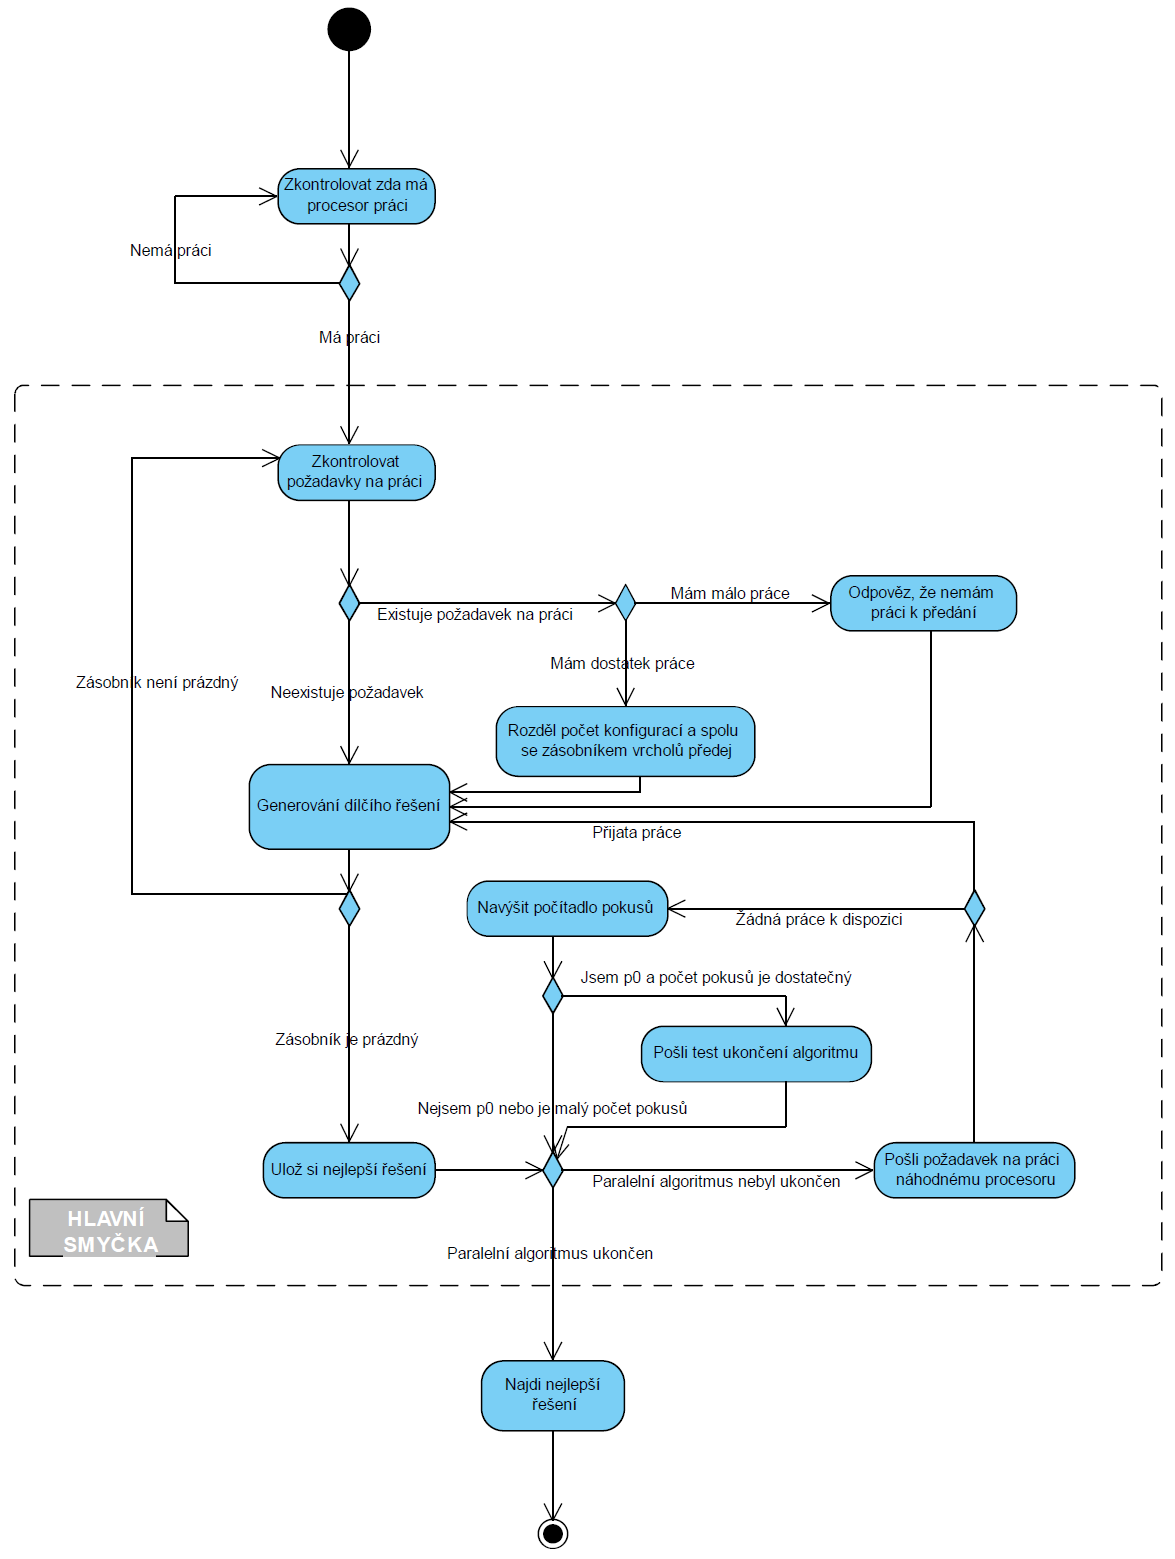
\includegraphics[scale=0.5]{while.jpg}
\caption{Hlavní smyčka paralelního algoritmu.}
\label{hlavniSmycka}
\end{figure}

\section{Návod pro vkládání grafů a obrázků do Latexu}

Nejjednodušší způsob vytvoření obrázku je použít vektorový grafický
editor (např. xfig nebo jfig), ze kterého lze exportovat buď
\begin{itemize}
\item postscript formáty (ps nebo eps formát) nebo
\item latex formáty (v~pořadí prostý latex, latex s~macry epic, eepic, eepicemu). Uvedené pořadí odpovídá růstu
komplikovanosti obrázků který formát podporuje (prostá latex macra
umožnují pouze jednoduché, epic makra něco mezi, je třeba
vyzkoušet).

\end{itemize}
Následující příklady platí pro všechny případy.

Obrázek v~postscriptu, vycentrovaný a na celou šířku stránky,
s~popisem a číslem. Všimnete si, jak řídit velikost obrazku.

Obrázek pouze vložený mezi řádky textu, bez popisu a číslování.\\


bez čísla a popisu.

Takhle jednoduše můžete poskládat obrázky vedle sebe.

Řídit velikost latexovskych obrázků lze příkazem
\begin{verbatim}
\setlength{\unitlength}{0.1mm}
\end{verbatim}
které mění měřítko rastru obrázku, Tyto příkazy je ale současně
nutné vyhodit ze souboru, který xfig vygeneroval.

Pro vytváření grafu lze použít program gnuplot, který umí generovat
postscriptovy soubor, ktery vložíte do Latexu výše uvedeným
způsobem.

\end{document}
